\chapter{Introducción a la lógica difusa}
\label{ch:fuzzyApendix}

La lógica difusa surge como una extensión de la lógica clásica para afrontar la realidad imprecisa de nuestro entorno. Mientras que la lógica tradicional solo admite valores binarios (verdadero o falso), en la lógica difusa cada afirmación puede matizarse con un grado de verdad entre 0 y 1. La capacidad de graduar la pertenencia a un concepto, como por ejemplo "barato" o "cercano", brinda a la lógica difusa la posibilidad de emular con más fidelidad el razonamiento humano. 

A continuación, se expondrán, de manera general, los elementos esenciales de la lógica difusa.

\section{Conjuntos difusos}
\label{apx:ConjuntosDifusos}

Un conjunto difuso introduce una función de membresía que asigna a cada elemento "x" un valor real entre 0 y 1, a diferencia de un conjunto clásico, cuya función indica si un elemento pertenece o no al conjunto. En la práctica, las funciones de membresía más utilizadas son las trapezoidales y las triangulares, debido a que se definen con pocos parámetros y describen con claridad regiones de pertenencia total y parcial. Además, su formulación matemática facilita el cálculo y la visualización. En la Figura~\ref{fig:FuncionesTrapezoidalTriangular} se puede ver un ejemplo de un conjunto trapezoidal y un conjunto triangular. 

\begin{figure}[H]
\centering
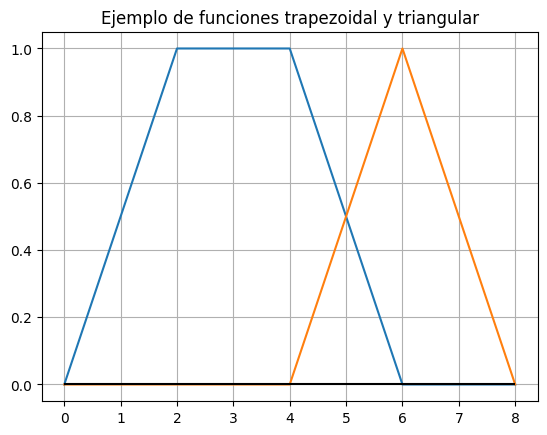
\includegraphics[width=.65\textwidth]{fig/Fuzzy/Ejemplo de funcion trapezoidal y triangular.png}
\caption{Ejemplo de funciones trapezoidal, en azul, y triangular, en naranja.}
\label{fig:FuncionesTrapezoidalTriangular}
\end{figure}

\section{Variables lingüísticas}
\label{apx:VariablesLing}

Una variable lingüística es un modo de nombrar información numérica usando palabras en lugar de cifras. Estas vienen definidas por un nombre, como por ejemplo "temperatura", el rango de valores que puede tomar, como por ejemplo de 0 a 35 \textdegree{}C y un conjunto de etiquetas, como por ejemplo, "fría", "templada" y "caliente". Cada etiqueta lleva asociado un conjunto, con su correspondiente función de membresía (triangular, trapezoidal, etc.). De esta manera, decir que la temperatura es "templada", no sería una verdad absoluta, sino que sería un valor real comprendido entre 0 y 1, como por ejemplo 0,6. Esto reflejaría cuantitativamente la pertenencia del dato dentro de esa categoría, en este caso que la temperatura sea templada.

\section{Proposiciones difusas}
\label{apx:ProposicionesDifusas}

Una proposición difusa es una afirmación del tipo: "variable ES término", por ejemplo, si la "distancia ES corta" o la "velocidad ES alta". Estas proposiciones no son ni verdaderas ni falsas de forma inequívoca, como pasaba en la lógica clásica, sino que devuelven un grado de verdad igual al valor de la función de membresía correspondiente. Estas proposiciones pueden ser proposiciones atómicas, si estas no se pueden subdividir en otras proposiciones, o proposiciones compuestas o moleculares, si están conformadas por una o más proposiciones atómicas. Un ejemplo de una proposición compuesta sería "distancia ES corta Y velocidad ES alta", que estaría formada por las proposiciones atómicas "distancia ES corta" y "velocidad ES alta".

\section{Reglas difusas}
\label{apx:ReglasDifusas}

Las reglas difusas son los enunciados condicionales que se emplean en lógica difusa para ligar expresiones imprecisas con términos lingüísticos. Por lo general, tienen la siguiente estructura: \texttt{IF <antecedente> THEN <consecuente>}, donde el antecedente puede ser una proposición atómica o una proposición compuesta y el consecuente asigna valores de pertenencia o una proposición atómica, dependiendo del modelo empleado. Por ejemplo, en el modelo Mamdani, el antecedente sería una proposición atómica o compuesta y el consecuente sería una proposición atómica, como por ejemplo, \texttt{IF velocidad alta AND distancia lejana THEN freno bajo}.

%Modelos difusos
\section{Modelos difusos}
\label{apx:ModelosDifusos}

Dentro de la lógica difusa se han desarrollado distintos modelos que definen cómo se representa el conocimiento, cómo se formulan las reglas y cómo se obtiene una salida a partir de las entradas. Cada modelo responde a necesidades distintas según el contexto de la aplicación: control de sistemas, predicción, clasificación, entre otros. A continuación se presentan algunos de los modelos más utilizados en lógica difusa.

\subsection{Modelo de Mamdani}
\label{apx:ModeloMamdani}

El modelo de Mamdani~\cite{MAMDANI19751} es el más conocido. Cada regla está formada por un antecedente, que puede ser una proposición atómica o una proposición compuesta, y por un consecuente, que es siempre una proposición atómica, con lo que una regla difusa siguiendo el modelo de Mamdani tiene la siguiente forma: \texttt{IF <antecedente> THEN <consecuente>}.

Para obtener una salida, primero se evalúa el antecedente. Si la regla difusa tiene una proposición compuesta y esta tiene un operador \texttt{AND}, se toma el valor mínimo entre los valores de pertenencia de las proposiciones atómicas que componen la proposición compuesta, por otro lado, si el operador fuera un \texttt{OR}, se toma el valor máximo entre los valores de pertenencia de las proposiciones atómicas de la proposición compuesta. El resultado de esta evaluación es el grado de activación de la regla.

Después, el grado de activación de la regla se emplea como límite superior para la salida, por lo que si un valor supera este umbral, se recorta al nivel del grado de activación. Una vez hecho esto para todos los puntos del dominio, se combinan todas las salidas obtenidas realizando, por ejemplo, el máximo punto a punto de los valores recortados.

Por último, con el área obtenida de combinar las salidas, se calcula el centroide de este para obtener la salida de la regla difusa (defuzzificación). 

\subsection{Modelo Tsukamoto}
\label{apx:ModeloTsukamoto}

El modelo de Tsukamoto~\cite{jang1997neurofuzzy} es parecido al de Mamdani, pero obliga a los conjuntos de salida a ser monótonos, es decir, que su función de pertenencia debe crecer o decrecer de forma continua sin cambiar de sentido. Esto permite que cada regla difusa dé como salida un valor directamente. Después, se realiza la media ponderada de todas las salidas de las reglas para obtener el valor de salida. De esta manera se evita el tener que realizar la defuzzificación de la salida.
\begin{comment}
\subsection{Modelo TSK}
\label{apx:ModeloTSKResumen}

El modelo TSK cambia los \texttt{THEN} empleados en otros modelos por funciones matemáticas. Al no necesitar defuzzificación, este modelo es más preciso y rápido que otros modelos.

En la siguiente sección se hablará de manera más distendida sobre este modelo.
\end{comment}
%Modelo TSK
\section{Modelo TSK (Takagi-Sugeno-Kang)}
\label{apx:ModeloTSK}

El modelo TSK (Takagi-Sugeno-Kang)~\cite{6313399} es una evolución del modelo de Mamdani, pero con un planteamiento mucho más matemático y orientado al rendimiento. La premisa que sigue este modelo es que, en lugar de emplear como salida un conjunto difuso, cada regla devuelva la salida como un valor numérico directamente a partir de una fórmula. Por ejemplo:

\begin{center}
    \texttt{IF Velocidad Alta AND Carga Media THEN \(\text{Salida} = 0.3 \times \text{Velocidad} + 0.6 \times \text{Carga} + 2\)}
\end{center}

Donde el antecedente corresponde con la proposición compuesta \texttt{Velocidad Alta AND Carga Media} y la salida es el resultado del cálculo de la fórmula \texttt{\(0.3 \times \text{Velocidad} + 0.6 \times \text{Carga} + 2\), suponiendo una velocidad de 100 y una carga de 50, la salida sería 62}

Para poder obtener una salida, primero se calcula el grado de activación de cada una de las reglas difusas que componen el sistema. Después se calcula el valor de cada una de las funciones de las reglas difusas. Por último, se calcula la salida como la media ponderada de todas las salidas de las funciones.

\begin{equation}
y = \frac{\sum_{i=1}^{n} w_i \cdot z_i}{\sum_{i=1}^{n} w_i}
\end{equation}

Donde:
\begin{itemize}
  \item $w_i$ es el grado de activación de la regla $i$, calculado a partir del antecedente de la regla difusa.
  \item $z_i$ es la salida de la regla $i$, obtenida evaluando la función del consecuente con los valores de entrada.
  \item $y$ es la salida global del sistema, obtenida como media ponderada de las salidas individuales.
\end{itemize}
\newpage
%Modelos difusos acumulativos: es un TSK que acumula los valores obtenidos por cada una de las reglas.
\section{Modelos difusos acumulativos}
\label{apx:ModelosDifusosAcumulativos}

El modelo difuso acumulativo~\cite{MUNOZVALERO2025113415} se basa en el modelo TSK, pero sustituye la fórmula que se emplea para calcular la salida de cada una de las reglas y en su lugar se utiliza un valor fijo. Además, cada regla del sistema contribuye de manera directa a la salida final, debido a que esta se calcula sumando los valores proporcionales de salida de cada una de las reglas difusas que tiene el sistema, en lugar de realizar la media ponderada de los valores de la salida de cada una de las reglas como en el modelo TSK clásico. Dicho esto, se puede reescribir la regla de ejemplo empleada en la sección del modelo TSK~\ref{apx:ModeloTSK} para que se adapte a este modelo cambiando la fórmula para calcular la salida por un número, por ejemplo, 60. De esta forma, la regla resultante es:

\begin{center}
   \texttt{IF Velocidad Alta AND Carga Media THEN 60} 
\end{center}

\noindent Para calcular los valores de salida de la regla del ejemplo se hace lo siguiente:

\begin{enumerate}
    \item Se calcula el grado de activación de la regla con la fórmula:
        \begin{equation}
            \alpha= \mu(\text{$A_1$ en $x_1$}) \times \mu(\text{$B_1$ en $y_1$})
        \end{equation}
    Donde:
        \begin{itemize}
            \item $\alpha$ es el valor del grado de activación de la regla difusa.
            \item $\mu(\text{$A_1$ en $x_1$})$ es el valor de la pertenencia para la proposición atómica A (\texttt{Velocidad Alta}) en $x_1$.
            \item $\mu(\text{$B_1$ en $y_1$})$ es el valor de la pertenencia para la proposición atómica B (\texttt{Capacidad media}) en $y_1$.
            \item $x_1$ es el valor conocido de la entrada para la velocidad en el punto 1.
            \item $y_1$ es el valor conocido de la entrada para la carga en el punto 1.
        \end{itemize}
    \item Empleando el valor de $\alpha$ y el valor del consecuente, en este caso 60, se calcula la contribución de la regla multiplicando el valor de $\alpha$ por 60.        \begin{equation}
            \mu_{R_1} = \alpha \times 60
        \end{equation}
    \item Si hubiera más reglas difusas, se seguiría el mismo procedimiento descrito en 1 y 2 para calcular la contribución de cada una de las reglas.
    \item Después de calcular la contribución de cada una de las reglas, estas se suman para obtener el valor de la decisión.
        \begin{equation}
            DV = \sum_{i=1}^n (\mu_{R_i})
        \end{equation}
    Para el caso del ejemplo, como solo tenemos una regla, el valor sería directamente el valor de contribución de la regla, por lo que \(DV=\alpha\times60\).
\end{enumerate}

Este es el modelo empleado por \acrshort{ROBIN} en el momento de redacción de este \acrshort{TFG}.